\chapter{OpenGL}

OpenGL是状态机一下子不好理解,如果从API层面来说就比较容易了,Pascal之父Nicklaus Wirth说过算法+数据结构=程序
,而OpenGL的API没有一个数据要求是结构的,\textbf{OpenGL has no data structures. None at all. The entire OpenGL API is made of functions, taking simple value-arguments, or at most pointers to C-strings or binary-blobs, but never pointers to data structures.}
状态机的表现就是通过Context来管理的,所有的API都在此基础上。

客户端与服务端也是OpenGL的一个重要2概念,一般把应用层看成客户端,硬件与驱动程序看成服务端,它们各自维护着各自的状态,某些API的调用就
跟这个概念有很大的关系,OpenGL的发展与优化也是因为客户端与服务端的角色与重要性产生变化的原因。

\section{Buffer}

Buffer概念在编程中很难直接对应于中文的字,它是一个很泛的概念,需要根据上下文与特定语境来分析,否则很容易理解错误。

\paragraph{FBO}

Frame Buffer Object帧缓冲区对象,它不是内存块,不实际存储数据,可比作画画中的画板,画画时需要挂载画布,在画布上进行绘图。
FBO就是画板,它需要attachment不同的画布才能继续操作。

\begin{itemize}
    \item {Color, 就是绘制的图像数据,即RGBA数据, 如使用Multiple Render Target技术,可能存在多个Color Attachment}
    \item {Depth,绘制图像的深度数据,一般用于判断物体的远近实现遮挡效果}
    \item {Stencil,渲染中的高级技术,就像印制中的模板一样,一般用于渲染时进行像素级别的提出与遮挡,如三维描边}
\end{itemize}

\begin{figure}[h]
    \centering
    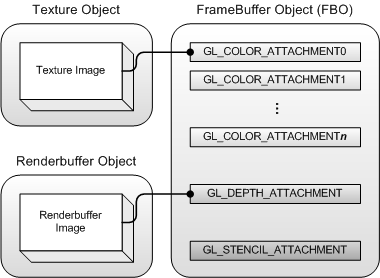
\includegraphics[width=\textwidth]{images/gl_fbo.png}
\end{figure}

这些attachment的画布具体就是两类数据Texture和RenderBuffer。一般情况下,就像画画时不能把两张画布放在一个画板上一样,texture和renderbuffer
也不能同时挂载一个FBO上。

\paragraph{Buffer Object}

就是存储图元primitive数据的地方, 上面说了客户端CPU与服务端GPU,随着角色的变化,由VertexArray内存到VertexBuffer Object(VBO)显存的发展,
也是由固定管线到可编程管线的变化,尽量减少数据的传输与方便数据更新。

\begin{lstlisting}
// TARGET = GL_ARRAY_BUFFER, GL_ELEMENT_ARRAY_BUFFER, 
// GL_TEXTURE_BUFFER, GL_PIXEL_PACK_BUFFER... 
// vertex position
glGenBuffer(1, &vboPos);
glBufferData(TARGET, size, data, GL_STREAM_DRAW);
// vertex texture Coordinate
glGenBuffer(1, &vboTex);
glBufferData(TARGET, size, data, GL_STREAM_DRAW);
// vertex index     
glGenBuffers(1, &vboIdx);
glBufferData(TARGET, size, data, GL_STREAM_DRAW);

// draw with no shader, only static data 
glBindBuffer(TARGET, vboPos);
glEnableClientState(TARGET);
glVertexPointer(3, GL_FLOAT, 0, NULL);

glBindBuffer(TARGET, vboTex);
glEnableClientState(TARGET);
glTexCoordPointer(2, GL_FLOAT, 0, NULL);

glBindBuffer(TARGET, vboIdx);
glDrawElements(GL_TRIANGLES, 6, GL_UNSIGNED_SHORT, NULL);
glBindBuffer(TARGET, 0); // index buffer 
glDisableClientState(TARGET); // vertex texture coordinate
glDisableClientState(TARGET); // vertex position
glBindBuffer(TARGET, 0); // 
glBindBuffer(TARGET, 0); // 

// draw with shader
glBindBuffer(TARGET, vboPos);
glEnableVertexAttribArray(location1);
glVertexAttribDivisor(location1); // multi-instance drawing
glVertexAttribPointer(location1, 2, GL_FLOAT, GL_FALSE, 0, 0);

glBindBuffer(TARGET, vboTex);
glEnableVertexAttribArray(location2);
glVertexAttribPointer(location2, 2, GL_FLOAT, GL_FALSE, 0, 0);

glBindBuffer(TARGET, vboIdx);
glDrawElements(GL_TRIANGLES, 6, GL_UNSIGNED_SHORT, NULL);

glDisableVertexAttribArray(location1); 
glDisableVertexAttribArray(location2);
glBindBuffer(TARGET, 0);  
glBindBuffer(TARGET, 0);  

// after bind buffer, and update data stytle 
// one 
glBufferData(TARGET, ...);
// two 
glBufferSubData(TARGET, ...);
// three 
glMapBufferRange(TARGET, ...);
glUnmapBuffer(TARGET, ...);
\end{lstlisting}

\paragraph{VAO}

与FBO一样,是Buffer Object的容器,是为管理数据而引入的一个状态容器,把内存数据Buffer Object放在一个对象中。这样处理的目的是
一个渲染流程有多份不同渲染逻辑,Context可能进行切换,但数据可能是一份,为了共享数据,每次渲染时直接使用vao,而不需要每次
都去处理vbo的数据绑定流程。 

\begin{lstlisting}
glGenBuffers(1, &vboPos);
glBingBuffer(GL_ARRAY_BUFFER, vboPos);
glBufferData(GL_ARRAY_BUFFER, sizeof(dataPos), dataPos, GL_STREAM_DRAW);

glGenBuffers(1, &vboTex);
glBingBuffer(GL_ARRAY_BUFFER, vboTex);
glBufferData(GL_ARRAY_BUFFER, sizeof(dataTex), dataTex, GL_STREAM_DRAW);

glGenBuffers(1, &vboIdx);
glBingBuffer(GL_ARRAY_BUFFER, vboIdx);
glBufferData(GL_ARRAY_BUFFER, sizeof(dataIdx), dataIdx, GL_STREAM_DRAW);

// 
glGenVertexArrays(1, &vao);
glBindVertexArray(vao);

glBindBuffer(GL_ARRAY_BUFFER, vboPos);
glEnableVertexAttribArray(location1)
glVertexAttribPointer(location1, 2, GL_INT, GL_FALSE, 0, 0);

glBindBuffer(GL_ARRAY_BUFFER, vboTex);
glEnableVertexAttribArray(location2)
glVertexAttribPointer(location2, 2, GL_INT, GL_FALSE, 0, 0);

glBindBuffer(GL_ELEMENT_ARRAY_BUFFER, vboIdx);

glBindVertexArray(0);

glBindBuffer(GL_ELEMENT_ARRAY_BUFFER, 0);
glBindBuffer(GL_ARRAY_BUFFER, 0);

// use 
glBindVertexArray(vao);
glDrawElements(GL_TRIANGLES, 6, GL_UNSIGNED_SHORT, 0);
glBindVertexArray(0);
\end{lstlisting}

\paragraph{PBO}

Pixel Buffer Object, 

\section{Coordinate}

OpenGL是右手系坐标

\subsection{Ordinary Coordinate}
普通坐标,

\subsection{Homogeneous Coordinate}
齐次坐标系,为了计算的一致性,使用矩阵可以方便表示旋转,缩放,但是平移就不行了。进行升维操作,
可以把2维扩展维3三维,三维扩展为四维,这样就能保证旋转,缩放,平移都以矩阵形式来表示。

齐次坐标系是计算机图形学的基础,能够明确区分向量和点,同时也易于进行仿射(线性)几何变换。

\subsection{Coordinate Space}
坐标空间是一个相对概念,

\paragraph{Modle Space}
物体空间坐标,局部空间。把物体从局部空间放到世界空间中,需要一个Model Matrix的变换过程。

\paragraph{World Space}
世界空间,就是整个场景的参考坐标系。把场景放到摄像机空间需要一个View Matrix的变换过程。

\paragraph{Eye-Camera Space}
摄像机空间,观察者所在坐标空间中。从观察空间到裁剪空间需要一个Projection Maxtrix的变换过程。

\paragraph{Clip Space}
裁剪空间,
会进行Perspective division透视除法,为了透视效果。

\paragraph{NDC Space}
视口空间, Normalized Device Coordinate Space, 这里与设备进行规范化转换。
需要一个Viewport Matrix转换到屏幕空间中。

OpenGL的坐标原点是左下角,Vulkan的坐标原点是左上角。在共享shader时,就需要注意两种的区别了。


\paragraph{Screen Space}
屏幕空间


\section{Shader}

\subsection{screen space derivative}
屏幕空间偏导数
GPU always evaluate fragment/pixel shaders on 2x2 blocks of pixels at a time.

use this techniques for rendering antialiased lines

\begin{figure}[h]
    \centering
    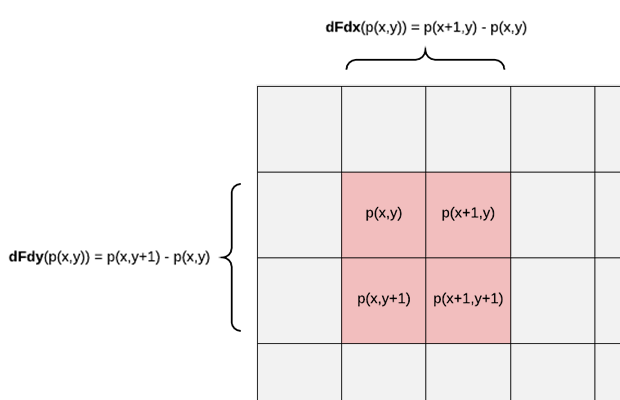
\includegraphics[width=\textwidth]{images/Shader-Derivatives.png}
\end{figure}

antialiasing,AA抗锯齿,对于一张纹理,给定UV坐标后,不仅仅是直接采样,还要考虑周围方形
区域内采样的结果,这个区域就是ddx和ddy给定的区域,在shader中调用texture时,后台进行了处理,
在一些高级的profiles中,还是允许自定义滤波窗口大小的

mipmap,在屏幕空间中,纹理坐标变换剧烈,Derivatives are used during texture sampling to
select the best mipmap level.

\paragraph{fwidth}
GLSL中,fwidth函数返回的是X和Y方向偏导数的绝对值的和,而单方向的偏导数可以通过ddx和ddy获得

注意,这些函数与像素有关,只能在fragment/pixel shader中使用


\section{RenderPass}

Render Pass定义为一个渲染步骤。如有一个很多不同材质的球体的场景需要渲染,就可以声明一个render pass给所有球使用,因为对每一个球体,渲染结果都会输出到同一个FrameBuffer的Attachment上,所以流程上是一样的。

如果说Buffer的数据可以供所有shader使用,那么在render pass中就是更加定制化的渲染,

每个pass通常对应的渲染流程中不同阶段【相同阶段通常会使用MRT,或硬件不支持,需要多个Pass;或渲染目标size不一样,也需要多个pass来渲染】。实际意义是对一个Mesh渲染多遍,是对材质抽象的一种解释,一个Technique里会包含一个或多个Pass,如DeferredLighting流程里面一个物体就需要2个Pass,一个用来计算Z,一个用来lighting;如果有阴影,又需要一个Pass;如果需要精细反射图,需要一个反射的Pass。引擎一般会把状态类似的不同Mesh的Pass一起渲染, 用Pass对材质进行排序。


\section{Technique Artist}
技术美术

\section{3D Render Library}

\subsection{Render Engine}

\textbf{OpenSceneGraph}

\textbf{bgfx}

\textbf{Armory Engine}\cite{Armory}, Armory is an open-source 3D engine focused on portability, minimal footprint and performance. The renderer is fully scriptable with deferred and forward paths supported out of the box.Written in C, Haxe and WebAssembly, structured as a data-driven engine.

\textbf{UPBGE}\cite{upbge}, is an open-source 3D game engine forked from old Blender Game Engine, deployed with Blender itself. This unified workflow is its main strength as you can make your game from start to end without leave UPBGE.

\textbf{three.js}

\textbf{Babylon.js}


\chapter{Vulkan}

vulkan是控制GPU设备的API,是OpenGL下一代且更底层的API,由OpenGL驱动提供的功能都需要自己实现,包括,同步,进度,内存管理等。
所以vulkan是适合大型复杂的图形渲染,定制性要求很高,OpenGL提供不了的功能。

既然是API,它相比OpenGL的状态机,更符合面向对象设计,与DirectX类似,是C语言的接口,这算是OpenGL切换到Vulkan最直接的感受。
从应用视角来看,以前很多由Runtime/Driver实现的功能,都开始转型接口控制,给应用层更大的定制性,对特定的业务与跨平台和不同的
运行环境都有很好的适配性。

\section{Memory}
Vulkan延续OpenGL的Host-Device设计模型,将CPU与GPU看成是一个异步执行的过程,这样CPU可以多线程提供数据给GPU使用。
这也是Vulkan是基于现代GPU渲染模型的一个抽象包装,相比CPU的多缓存与串行执行模型,GPU是高并发和高延迟。

Vulkan内存分为Host与Device两大类,Host Memory是使用vulkan主机可访问的内存,又称系统内存。Device Memory可由
GPU Local Memory显存和Host Local Memory部分系统内存组成。对CPU就是VkBuffer数据源,对GPU就是
VkDeviceMemory。

\subsection{Resource}

vulkan的操作基于数据,所有data都存储在resources中,它们被后台内存管理着,构建这些资源大致有两步
\begin{itemize}
    \item {resource is created, ex, vkCreateBuffer}
    \item {resource needs to be backed by memory, 允许应用程序管理内存}
\end{itemize}

\paragraph{buffers}

线性存储块,可拥有存储任何的数据,它同样可以存储图像数据

\paragraph{images}

图像,具有结构性,类型,格式的固定数据


\section{Pipeline}
OpenGL的所有状态都由OpenGL的VM进行管理,而Vulkan相反,把所有渲染状态都放在一个VkPipeline对象上。
包含了所有可编程programable渲染状态和所有的固定功能fixed-function状态。可见VkPipeline的设置非常
繁琐。

\paragraph{ShaderModule}
VkShaderModule是最核心的一个,在VkGraphicPipeline中必不可少,Vulkan没有指定Shader语言,定义了一种
二进制的中间格式SPIR-V,可实时和离线编译成文件,GPU驱动程序再将代码编译成GPU-Specific的汇编代码。

这段相当于OpenGL中的glUseProgram逻辑。

\paragraph{PipelineLayout}
它由DescriptorSetLayout与DescriptorSet,Descriptor组成。
它们的作用就是GLSL中的Attribute,Uniforms,Varying这些作用。

\paragraph{Input Assembly State}
指定图元的拓扑topology方式,与OpenGL中的glDrawElements中的mode参数。

\paragraph{Rasterization}
Pipeline对象需要显式指定光栅化操作中的状态,属于光栅化模块的参数配置,如CullMode,FrontFace的winding
,depth的bias,linewidth等。

\paragraph{Multisampling}
多重采样

\paragraph{Blend}
混合只发生于color attachment。混合参数也是参数配置

\paragraph{RenderPass}
是指一组attachment,Subpass和Subpass之间的依赖,Pipeline对象引用了一个VkRenderPass对象

\subsection{CommandBuffer}



\section{同步}
现代图形API与传统API就是硬件带来的并行优势,而并行必然与资源同步关联在一起。同步本质上是图形硬件的并行机制在软件层面
的体现,需要对GPU的并行机制甚至硬件架构有一定的了解才能彻底理解同步。与多核CPU下的多线程编程的线程同步类似,同步的
原语种类较多,使用复杂,至少有两种,而Vulkan有四种,同步粒度不同,使用场景不同,同步最难的是不能很好的优化。

\subsection{GPU并行机制}
从API层面来看,Command是依次执行的,GPU是在执行时将Queue中的指令同时分发给GPU多核中的Pipeline执行,这就是GPU并行计算的机制,而这种并行是不会保证执行的
顺序的,原因有:
\begin{itemize}
    \item \text{Command在Command Buffer中顺序并不代表GPU内部执行顺序}
    \item \text{提交到同一Command Queue中不同Command Buffer的顺序不代表GPU内部执行顺序}
    \item \text{不同Command Queue提交的顺序不代表GPU内部执行顺序}
\end{itemize}
现代的图形硬件中都有基本的三种类型Command Queue:
\begin{itemize}
    \item \text{Transfer Queue, 用于从CPU向GPU传输数据,只执行Transfer命令}
    \item \text{Compute Queue,可执行Compute和Transfer指令}
    \item \text{Graphics Queue,执行图形渲染,可执行所有的GPU命令}
\end{itemize}
而GPU内部是高度管线化的,每种Command Queue分别对应不同的Pipeline Stage,而同步就是在这些Pipeline Stage中。
\paragraph{Transfer}
Transfer
\paragraph{Compute}
Indirect Draw, Compute Shader
\paragraph{Graphics}
Indirect Draw, Vertex Input, Vertex Shader, Tessellation Control Shader, 
Tessellation Evaluation Shader, Geometry Shader, Fragment Shader, Color Attachment Output

    
\subsection{GPU Cache}
与CPU缓存类似,

\subsection{什么是图形API的同步}
从同步的硬件与从同步的内容来分析,有四种情况:
\subsubsection{CPU And GPU}

\subsubsection{GPU Internal}

\subsubsection{Command}
指令同步,执行依赖,GPU执行指令时完全是并行的,并行的边界是全局的,这样当执行的指令有逻辑的依赖时就需要指令同步。 
\subsubsection{Data}
数据同步,数据依赖,从一个Pipeline Stage到另一个时需要数据同步。

\subsection{同步原语}
传统的都是放在Runtime/Driver中隐式实现了,这种实现对应用层来说简单易用,但是不容易扩展,具有通用性,启发式,预判的
一些限制。

Vulkan的同步是最全面的,最接近硬件,也是最复杂的。

Fence和Semaphores即时数据同步也是指令同步,是粗粒度的同步原语,Fence是Host与Device之间,Semaphores是Queue之间。


\subsubsection{Fence}
用于Device向Host传达任务完成的事件,即CPU与GPU之间的同步,典型的场景是通过Fence等待某个GPU Queue中的所有的Command
执行完成。在CPU端通过vkGetFenceStatus轮询获取Fence状态,不能设置完成事件回调。 

\subsubsection{Semaphores}
属于GPU内部的同步, 典型的场景是渲染时确定每个资源完成的信号来通知下一步, 也可在多个GPU Queue中进行同步,
如Graphics中等待Compute资源的完成。

\subsubsection{Pipeline Barrier}
在同一Queue中同步,有两个参数,Source Pipeline Stage和Destinition Pipeline Stage。设置Barrier后,所有的Source
都保证在Destinition之前,在Source与Destinition之间的Stage越多并行度越高。

Barrier可以在RenderPass之间,也可以是RenderPass的SubPass内部,此时的SubPass是自依赖的

\subsubsection{Event}
Event可以看成是分离的Barrier,控制粒度更细,通过vkCmdSetEvent指定Source,通过vkCmdWaitEvent指定Destinition
